\documentclass{article}
\usepackage[paperwidth=84.1cm,paperheight=118.9cm,margin=0cm]{geometry}
\usepackage{fontspec}
\usepackage{unicode-math}
\usepackage[brazilian]{babel}
\usepackage{ragged2e}
\usepackage{graphicx}
\usepackage{tikz}
\usetikzlibrary{arrows.meta}
\usepackage{qrcode}
\usepackage[hidelinks]{hyperref}
\setmainfont{Arial}
\setsansfont{Arial}
\setmathfont{latinmodern-math.otf}
\hypersetup{pdftitle={Algoritmos Exatos Para o Problema de Visita de Polígonos},pdfauthor={Gabriel Freire Ushijima; Ernesto G. Birgin},pdfsubject={34º SIICUSP, IME-USP}}
\pagestyle{empty}
\setlength{\parindent}{0pt}
\setlength{\parskip}{0.24em}
\definecolor{Ink}{HTML}{142D38}
\definecolor{Muted}{HTML}{47616A}
\definecolor{Accent}{HTML}{CF5A20}
\definecolor{Pale}{HTML}{EEF4F1}
\definecolor{Rule}{HTML}{C5D3CF}
\definecolor{MapDark}{HTML}{102C38}
\definecolor{Route}{HTML}{FFAD66}
\definecolor{FirstVisit}{HTML}{81D864}
\definecolor{LastVisit}{HTML}{1F7A73}
\newsavebox{\posterbox}
% Named, measured blocks make overflow checks reproducible after each edit.
\newcommand{\block}[5]{%
  \node[anchor=north west,inner sep=0] at (#2,#3) {%
  \sbox{\posterbox}{\begin{minipage}[t]{#4cm}\RaggedRight #5\end{minipage}}%
  \typeout{POSTERBLOCK #1 x=#2 y=#3 w=#4 h=\the\dimexpr\ht\posterbox+\dp\posterbox\relax}%
  \usebox{\posterbox}};}
\newcommand{\head}[2]{{\sffamily\bfseries\fontsize{44}{51}\selectfont\color{Accent}#1.\hspace{0.45cm}\color{Ink}#2\par}}
\newcommand{\bodytext}{\sffamily\mdseries\fontsize{28}{34}\selectfont\color{Ink}}
\newcommand{\bodymuted}{\sffamily\mdseries\fontsize{28}{34}\selectfont\color{Muted}}
\newcommand{\smalltext}{\sffamily\mdseries\fontsize{23}{28}\selectfont\color{Muted}}
\newcommand{\tagtext}{\sffamily\bfseries\fontsize{25}{30}\selectfont\color{Accent}}
\newcommand{\metric}{\sffamily\bfseries\fontsize{66}{72}\selectfont\color{Accent}}
\begin{document}
\begin{tikzpicture}[remember picture,overlay,shift={(current page.north west)},x=1cm,y=-1cm]
  \fill[white] (0,0) rectangle (84.1,118.9);
  \fill[Ink] (0,0) rectangle (84.1,0.55);
  % Crop the SIICUSP image's white margins so the visible marks align by height.
  % The IME and SIICUSP marks are both 6.643 cm tall; FAPESP spans their row.
  \block{ime-logo}{67.686}{3.938}{5.015}{\centering
\includegraphics[height=6.643cm]{figures/ime-usp-vertical-logo.png}}
  \block{event-logo}{73.201}{3.938}{7.899}{
\includegraphics[trim={33bp 56bp 33bp 79bp},clip,width=\linewidth]{figures/siicusp34-logo-pt.png}}
  \block{funding-logo}{67.686}{11.6}{13.414}{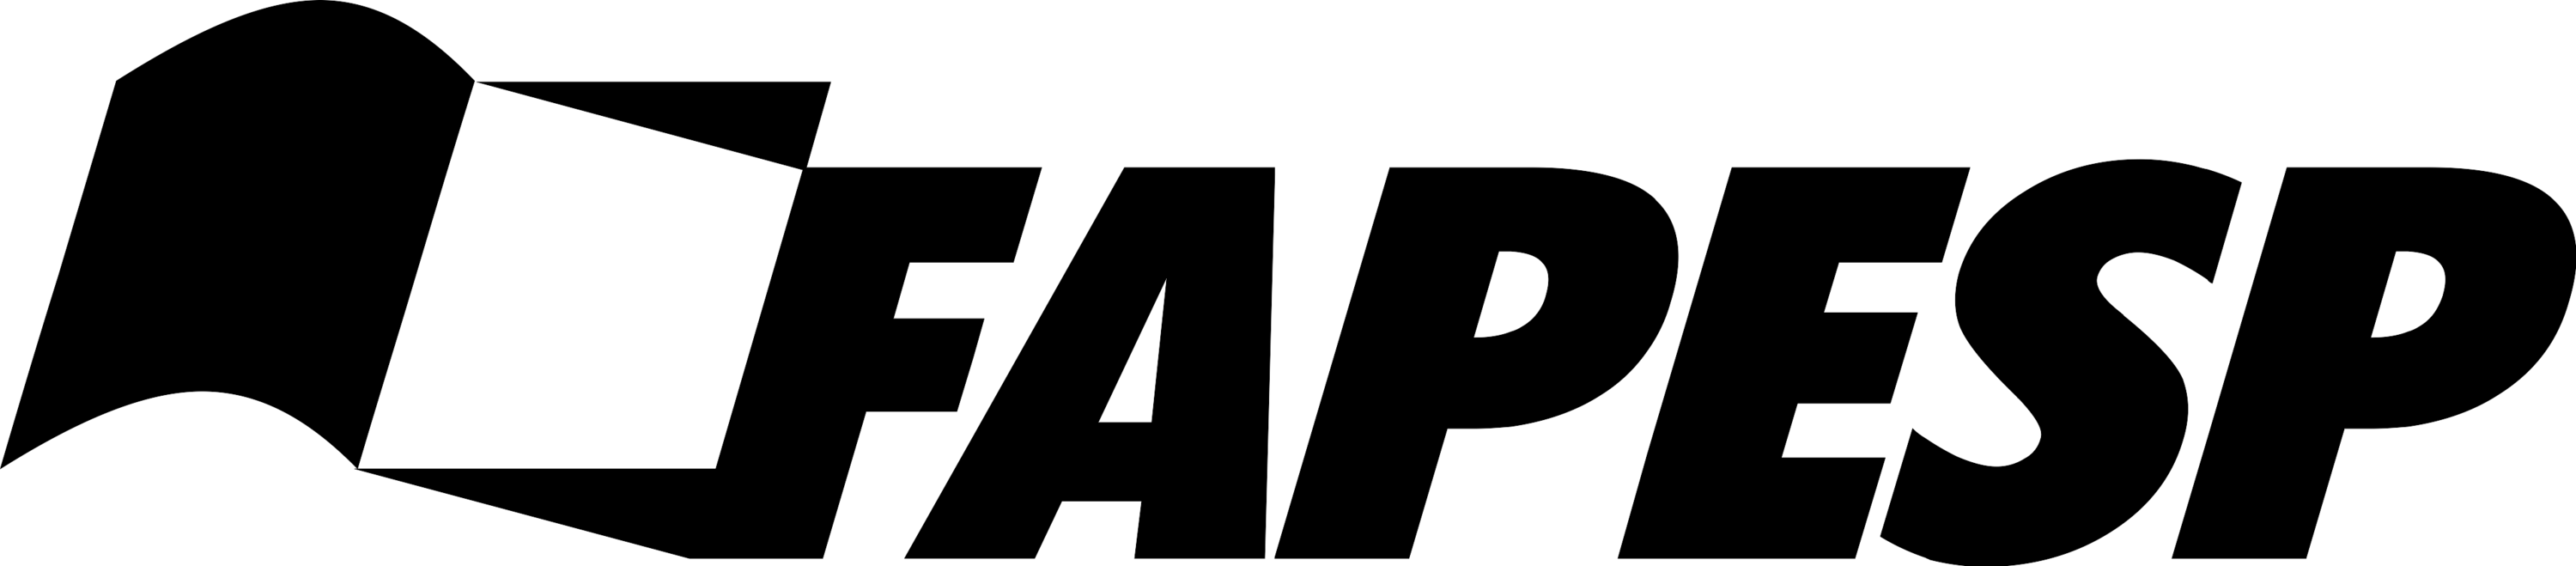
\includegraphics[width=\linewidth]{figures/fapesp-logo.png}}
  \block{funding}{67.686}{15.144}{13.414}{\raggedleft\sffamily\fontsize{17}{21}\selectfont\color{Muted}Processo 2025/13861-1\par}
  \block{title}{3}{4.4}{49.2}{\sffamily\bfseries\fontsize{90}{98}\selectfont\color{Ink}Algoritmos Exatos Para o\\Problema de Visita de Polígonos}
  \block{subtitle}{3}{11.3}{49.2}{\sffamily\fontsize{34}{41}\selectfont\color{Muted}Determinando caminhos mínimos para visitar regiões difíceis}
  \block{author}{3}{13.68}{37}{\sffamily\bfseries\fontsize{48}{55}\selectfont\color{Ink}Gabriel Freire Ushijima\par\vspace{0.08cm}\mdseries\fontsize{23}{27}\selectfont\color{Muted}\href{mailto:gabriel_ushijima@usp.br}{gabriel\_ushijima@usp.br}}
  \block{advisor}{30}{13.68}{51.1}{\sffamily\bfseries\fontsize{48}{55}\selectfont\color{Ink}Ernesto G. Birgin \mdseries(Orientador)\par\vspace{0.08cm}\fontsize{23}{27}\selectfont\color{Muted}\href{mailto:egbirgin@ime.usp.br}{egbirgin@ime.usp.br}}
  \draw[Rule,line width=1.1pt] (3,17.0) -- (81.1,17.0);
  % Section 1 uses one half-page column; its problem diagram has two inputs and one generalization.
  \block{intro-head}{3}{18.3}{38.2}{\head{1}{Introdução}}
  \block{intro-context}{3}{20.67}{38.2}{\bodytext A instância da USP tem 51 regiões. A rota começa e termina no mesmo ponto, junto à entrada do IME: 4,97 km em 8,77 s numa thread. No TPP de ordem livre, o solver escolhe a ordem e o ponto de contato em cada região.}
  \fill[Pale,rounded corners=0.22cm] (3,26.0) rectangle (20.4,31.35);
  \draw[Rule,line width=1.0pt,rounded corners=0.22cm] (3,26.0) rectangle (20.4,31.35);
  \block{tsp}{3.55}{26.35}{16.3}{{\sffamily\bfseries\fontsize{27}{32}\selectfont\color{Accent}TSP}\par\vspace{0.10cm}\bodytext Menor ciclo que visita um conjunto de pontos.}
  \fill[Pale,rounded corners=0.22cm] (3,32.1) rectangle (20.4,38.1);
  \draw[Rule,line width=1.0pt,rounded corners=0.22cm] (3,32.1) rectangle (20.4,38.1);
  \block{tpp}{3.55}{32.45}{16.3}{{\sffamily\bfseries\fontsize{27}{32}\selectfont\color{Accent}TPP}\par\vspace{0.10cm}\bodytext Menor caminho que parte de $s$, visita uma sequência de polígonos em ordem e chega em $t$.}
  \fill[Accent!7,rounded corners=0.24cm] (22.8,26.0) rectangle (41.1,38.1);
  \draw[Accent!65,line width=1.2pt,rounded corners=0.24cm] (22.8,26.0) rectangle (41.1,38.1);
  \block{free-order}{23.45}{29.0}{17.0}{{\tagtext TPP de ordem livre}\par\vspace{0.14cm}\bodytext Menor caminho que parte de um ponto $s$, visita um conjunto de polígonos e chega em um ponto $t$.\par\vspace{0.10cm}\bodytext\bfseries Esse é o problema que resolvemos.}
  \draw[Accent,line width=1.8pt,-{Stealth[length=3mm]}] (20.4,28.65) -- (22.7,29.15);
  \draw[Accent,line width=1.8pt,-{Stealth[length=3mm]}] (20.4,35.1) -- (22.7,34.8);
  \block{evolution}{3}{39.0}{38.2}{\smalltext\textbf{Complementando o resumo:} O texto submetido apresentava o caso não convexo com ordem fixa. Após a submissão, concluímos a extensão para ordem livre.}

  % Section 2 receives the full right half-column.
  \block{definitions-head}{42.7}{18.3}{38.4}{\head{2}{Trabalhos anteriores}}
  \block{prior-work}{42.7}{21.0}{38.4}{\tagtext Um subproblema polinomial\par\vspace{0.06cm}\bodytext Dror et al. (2003) deram algoritmo polinomial para o TPP com polígonos convexos em ordem fixa, em $O(nk^2\log n)$. Tan e Jiang (2017) reduziram para $O(nk^2)$. Aqui, $k$ é o número de polígonos e $n$ a soma dos vértices.}
  \block{competition-story}{42.7}{27.4}{38.4}{\tagtext A ideia e a comparação\par\vspace{0.06cm}\bodytext Quando começamos, enumerar ordens e peças convexas com branch and bound parecia o passo natural. Fekete et al. (2026) [3] publicaram abordagem semelhante poucos meses depois. No artigo, o subproblema convexo é resolvido por SOCP com Gurobi; nós usamos um solver geométrico especializado. O objetivo passou a ser superar o resultado deles nas próprias instâncias: com outra coleção, não mediríamos diretamente essa diferença.}

  % The USP map and the branch-and-bound explanation share the next row.
  \block{map-head}{3}{42.6}{29.5}{\head{3}{A USP como instância}}
  \block{usp-map}{3}{45.0}{29.5}{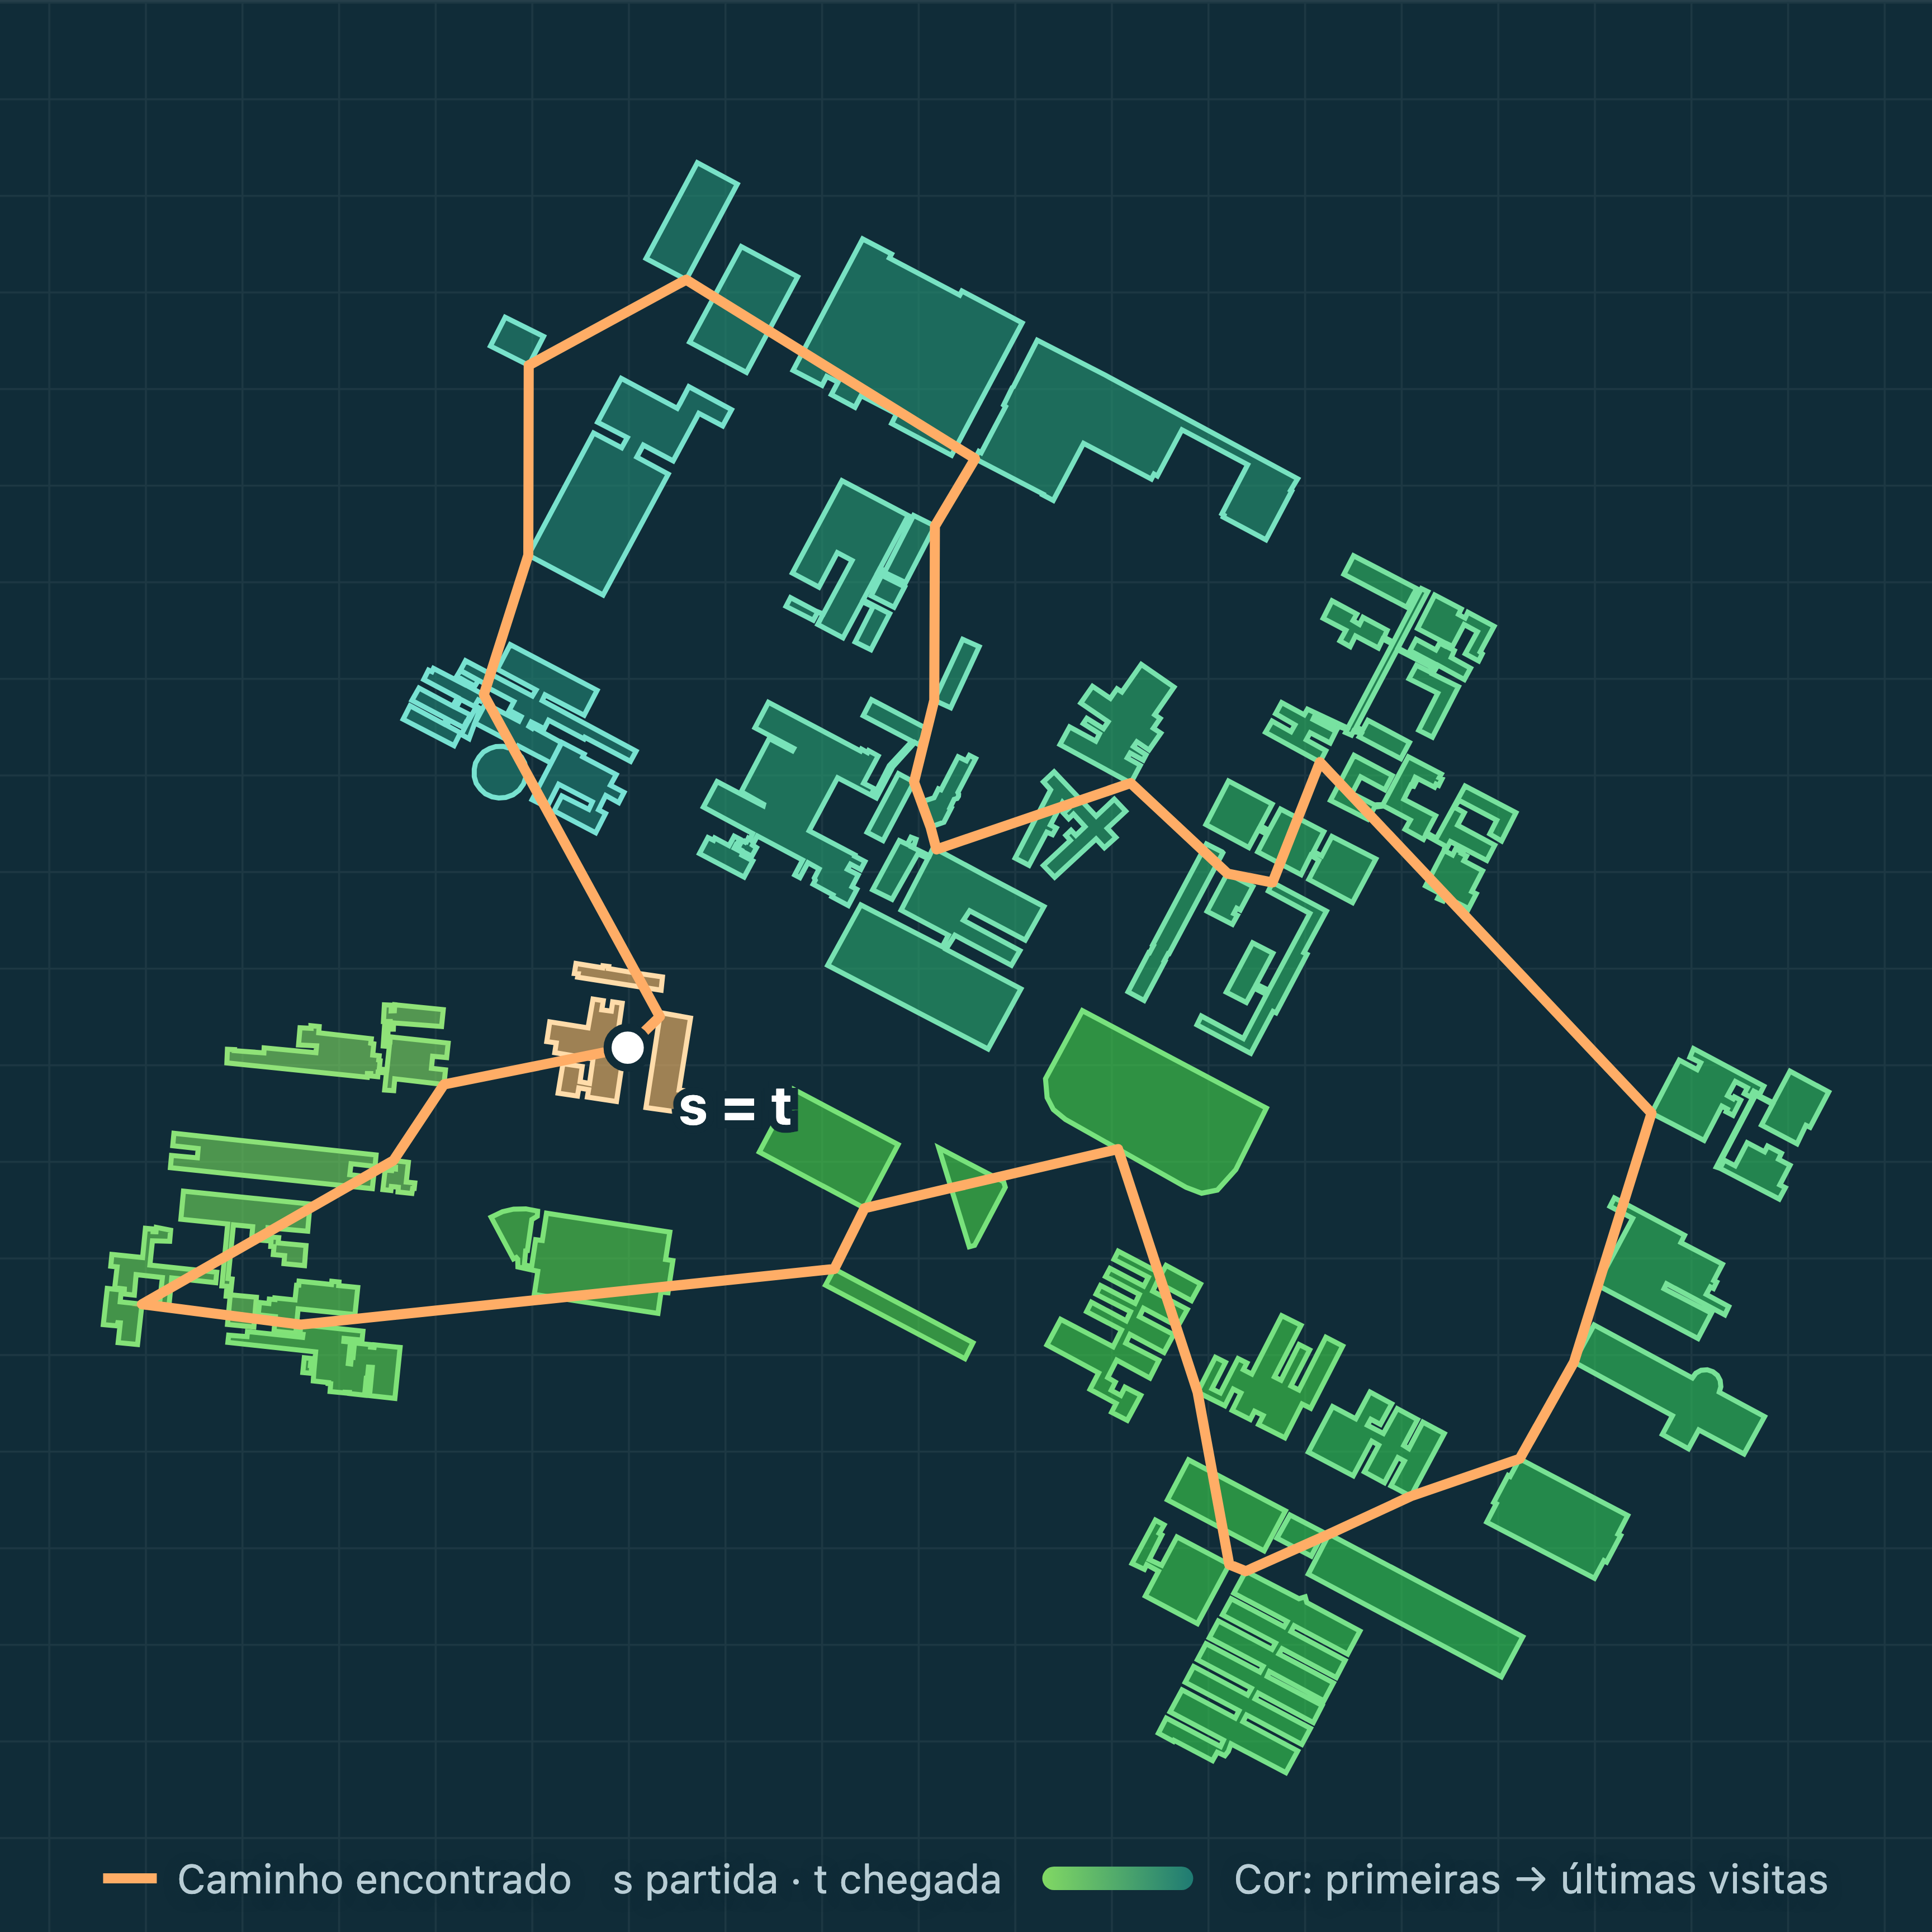
\includegraphics[width=\linewidth]{figures/usp-route-square.png}}
  \block{usp-context}{3}{75.0}{29.5}{\smalltext A região Google foi traçada manualmente no QGIS sobre OpenStreetMap. Regiões são alvos, não obstáculos; o modelo não inclui regras de voo.}

  \block{method-head}{35.5}{42.6}{45.6}{\head{4}{Buscar sem enumerar}}
  \block{brute-force}{35.5}{45.25}{37.8}{\bodytext Força bruta: testar ordens e escolhas de peças convexas. Usamos \textbf{Greene [4]} para decompor os polígonos.}
  % Real polygon and convex decomposition from usp-demo.js, building poli-civil.
  \begin{scope}[yshift=-2.3cm]
    % Generated from apps/siicusp34/data/usp-demo.js: buildings[poli-civil].
% Each fill is one recorded convex piece; dashed segments are shared internal edges.
\fill[LastVisit!22] (80.1486,43.9869) -- (80.7556,44.3064) -- (80.9800,43.8941) -- (79.8966,43.3108) -- (79.6736,43.7345) -- cycle;
\fill[LastVisit!22] (79.4980,45.1951) -- (80.0790,44.1220) -- (80.1486,43.9869) -- (79.6736,43.7345) -- (79.6024,43.8600) -- cycle;
\fill[LastVisit!22] (78.7408,44.7934) -- (79.4980,45.1951) -- (79.6024,43.8600) -- (78.1799,43.1000) -- cycle;
\fill[LastVisit!22] (78.7408,44.7934) -- (78.1799,43.1000) -- (77.5796,44.2135) -- (78.3347,44.6034) -- cycle;
\fill[LastVisit!22] (78.5750,45.1004) -- (78.7408,44.7934) -- (78.3347,44.6034) -- (78.1907,44.8627) -- cycle;
\fill[LastVisit!22] (78.5750,45.1004) -- (78.1907,44.8627) -- (77.4773,44.4873) -- (75.8200,47.5884) -- cycle;
\fill[LastVisit!22] (77.7184,48.6000) -- (79.3733,45.5315) -- (78.5750,45.1004) -- (75.8200,47.5884) -- cycle;
\draw[Muted!75,densely dashed,line width=1.0pt] (80.1486,43.9869) -- (79.6736,43.7345);
\draw[Muted!75,densely dashed,line width=1.0pt] (79.4980,45.1951) -- (79.6024,43.8600);
\draw[Muted!75,densely dashed,line width=1.0pt] (78.7408,44.7934) -- (78.1799,43.1000);
\draw[Muted!75,densely dashed,line width=1.0pt] (78.7408,44.7934) -- (78.3347,44.6034);
\draw[Muted!75,densely dashed,line width=1.0pt] (78.5750,45.1004) -- (78.1907,44.8627);
\draw[Muted!75,densely dashed,line width=1.0pt] (78.5750,45.1004) -- (75.8200,47.5884);
\draw[LastVisit,line width=1.7pt] (77.7184,48.6000) -- (79.3733,45.5315) -- (78.5750,45.1004) -- (78.7408,44.7934) -- (79.4980,45.1951) -- (80.0790,44.1220) -- (80.1486,43.9869) -- (80.7556,44.3064) -- (80.9800,43.8941) -- (79.8966,43.3108) -- (79.6736,43.7345) -- (79.6024,43.8600) -- (78.1799,43.1000) -- (77.5796,44.2135) -- (78.3347,44.6034) -- (78.1907,44.8627) -- (77.4773,44.4873) -- (75.8200,47.5884) -- cycle;

  \end{scope}
  \block{partition-label}{75.1}{50.95}{5.9}{\centering\sffamily\fontsize{20}{24}\selectfont\color{Muted}Civil-POLI}
  \fill[Pale] (35.5,51.6) rectangle (81.1,60.3);
  \block{case-tag}{36.1}{52.4}{44.4}{\tagtext CASO 49\hspace{0.4cm}·\hspace{0.4cm}60 REGIÕES}
  \block{case-equation}{36.1}{54.1}{44.4}{\sffamily\fontsize{37}{44}\selectfont\color{Ink}$60!\prod_i p_i\approx1{,}56\times10^{117}$}
  \block{case-explanation}{36.1}{56.2}{44.4}{\smalltext Combinações formais ($p_i$: número de peças do polígono $i$).\par\textbf{Resolvido em 2,47 s, com uma thread.}\par O solver não enumerou esse espaço.}
  \block{branch-and-bound}{35.5}{61.4}{45.6}{\bodytext Cada nó guarda uma ordem parcial, por exemplo $s\to\mathrm{IF}\to\mathrm{Central}\to t$. Omitir regiões e usar fechos convexos relaxa o problema.}
  % A valid relaxation supplies L; a complete feasible path supplies U.
  \fill[Pale] (35.5,66.8) rectangle (57.8,69.8);
  \draw[Rule,line width=0.8pt] (35.5,66.8) rectangle (57.8,69.8);
  \fill[Accent!7] (58.3,66.8) rectangle (81.1,69.8);
  \draw[Rule,line width=0.8pt] (58.3,66.8) rectangle (81.1,69.8);
  \block{lower-bound}{36.0}{67.2}{21.3}{\tagtext LIMITE INFERIOR\par\smalltext relaxação $L$}
  \block{upper-bound}{58.7}{67.2}{21.9}{\tagtext ROTA VIÁVEL\par\smalltext incumbente $U$}
  \draw[Muted,line width=1.4pt,-{Stealth[length=3.5mm]}] (46.65,69.8) -- (46.65,70.5) -- (58.3,70.5) -- (58.3,71.1);
  \draw[Muted,line width=1.4pt] (69.7,69.8) -- (69.7,70.5) -- (58.3,70.5);
  \fill[Pale] (35.5,71.1) rectangle (81.1,73.0);
  \block{prune}{35.5}{71.25}{45.6}{\centering\sffamily\bfseries\fontsize{39}{47}\selectfont\color{Accent}$L\geq U-\varepsilon\ \Rightarrow\ \text{poda}$}
  \block{branch-label}{35.5}{73.6}{45.6}{\tagtext Se não puder podar, ramifique:}
  \fill[Pale] (35.5,74.6) rectangle (57.8,78.4);
  \draw[Rule,line width=0.8pt] (35.5,74.6) rectangle (57.8,78.4);
  \fill[Pale] (58.3,74.6) rectangle (81.1,78.4);
  \draw[Rule,line width=0.8pt] (58.3,74.6) rectangle (81.1,78.4);
  \block{insert-branch}{36.0}{74.9}{21.3}{\tagtext INSERIR\par\smalltext região em cada posição}
  \block{refine-branch}{58.7}{74.9}{21.9}{\tagtext REFINAR\par\smalltext fecho em peças convexas}
  \block{method-note}{35.5}{78.9}{45.6}{\smalltext Inserção e refinamento adaptados de [3]. Só um limite inferior válido justifica a poda.}
  % Results keep the comparison corpus and denominators explicit.
  \draw[Rule,line width=1.1pt] (3,80.8) -- (81.1,80.8);
  \block{results-head}{3}{81.6}{78.1}{\head{5}{Resultados no corpus de Fekete et al.}}
  \fill[white,rounded corners=0.30cm] (3,83.9) rectangle (61.6,93.9);
  \draw[Rule,line width=1.0pt,rounded corners=0.30cm] (3,83.9) rectangle (61.6,93.9);
  \draw[Route,line width=4.0pt] (3.3,83.95) -- (17.6,83.95);
  \draw[LastVisit,line width=4.0pt] (17.6,83.95) -- (32.25,83.95);
  \draw[FirstVisit,line width=4.0pt] (32.25,83.95) -- (46.9,83.95);
  \draw[Muted,line width=4.0pt] (46.9,83.95) -- (61.3,83.95);
  \draw[Rule,line width=0.8pt] (17.6,84.3) -- (17.6,93.5);
  \draw[Rule,line width=0.8pt] (32.25,84.3) -- (32.25,93.5);
  \draw[Rule,line width=0.8pt] (46.9,84.3) -- (46.9,93.5);
  \block{speedup}{3.7}{85.1}{13.0}{\metric 5,11×\par\vspace{0.2cm}\bodytext\textbf{Speedup mediano}\par\smalltext Fekete / nosso solver, nas 550 instâncias concluídas por ambos.}
  \block{solved}{18.3}{85.1}{13.0}{\metric 558 / 558\par\vspace{0.2cm}\bodytext\textbf{Buscas concluídas}\par\smalltext O solver concluiu a busca nos 558 casos.}
  \block{under-ten}{32.95}{85.1}{13.0}{\metric 477 / 558\par\vspace{0.2cm}\bodytext\textbf{Em menos de 10 s}\par\smalltext Tempo de solver em uma thread por instância.}
  \block{faster}{47.6}{85.1}{13.0}{\metric 492 / 550\par\vspace{0.2cm}\bodytext\textbf{Instâncias mais rápidas}\par\smalltext Nosso solver foi mais rápido no conjunto comum concluído.}
  \block{result-explanation}{63.1}{84.1}{18.0}{\bodytext Rodamos as instâncias do artigo por até 6 h. Nosso solver concluiu 558/558; o de Fekete, 550/558. Tempo e speedup usam os 550 casos concluídos por ambos.}
  \fill[Pale] (3,94.6) rectangle (81.1,98.2);
  \block{conclusion-label}{3.6}{95.85}{10.4}{\tagtext CONCLUSÃO}
  \block{conclusion}{15}{94.95}{65.6}{\bodymuted Nas instâncias de Fekete, nosso solver foi mais rápido em 492/550 casos (mediana 5,11×). Nos pontos de contato, o P95 da distância até a região foi 0 m no nosso solver e 9,31 μm no de Fekete (16.303 vs. 15.883 visitas).}
  % Open questions are omitted in this compact proposal.
  \block{app-head}{3}{99.2}{18.5}{\head{6}{Tente você mesmo!}}
  \block{app}{21.5}{99.3}{51.5}{\bodytext Explore três desafios, mais de 500 instâncias e a simulação do algoritmo, passo a passo, no app.}
  \block{app-link}{21.5}{102.2}{51.5}{\sffamily\fontsize{20}{24}\selectfont\color{Muted}\href{https://yushipy.github.io/TouringPolygons/apps/siicusp34/}{yushipy.github.io/TouringPolygons/apps/siicusp34/}}
  \block{qr}{74.6}{98.3}{6.5}{\qrcode[level=H,height=6.5cm]{https://yushipy.github.io/TouringPolygons/apps/siicusp34/}}
  % References and credits; the digital PDF keeps live links.
  \draw[Rule,line width=0.8pt] (3,110.6) -- (81.1,110.6);
  \block{references-left}{3}{111.0}{32.0}{\sffamily\fontsize{22}{27}\selectfont\color{Muted}\textbf{Referências}\par
  [1] Dror et al. \href{https://doi.org/10.1145/780542.780612}{\emph{Touring a Sequence of Polygons}}. STOC, 2003.\par
  [2] Tan; Jiang. \href{https://doi.org/10.1007/978-3-319-55911-7_44}{\emph{Efficient Algorithms for Touring a Sequence of Convex Polygons and Related Problems}}. TAMC, 2017.\par
  [3] Fekete et al. \href{https://doi.org/10.4230/LIPIcs.SoCG.2026.46}{\emph{A Branch-and-Bound Algorithm for the Traveling Salesman Problem with Difficult Neighborhoods}}. SoCG, 2026.}
  \block{references-right}{37}{111.0}{28.2}{\sffamily\fontsize{22}{27}\selectfont\color{Muted}
  [4] Greene. \emph{The Decomposition of Polygons into Convex Parts}. Computational Geometry, 1983.\par
  O autor declara não haver conflito de interesses.}
\end{tikzpicture}
\end{document}
